\documentclass[11pt,a4paper]{article}

\usepackage[top=2cm,bottom=2cm,left=2.5cm,right=2.5cm]{geometry}
\usepackage{amsmath,amssymb}
\usepackage{booktabs}
\usepackage{multirow}
\usepackage{xcolor}
\usepackage{hyperref}
\usepackage{listings}
\usepackage{caption}
\usepackage{subcaption}
\usepackage{pgfplots}
\usepackage{pgfplotstable}
\usepackage{tikz}
\usepackage{titlesec}
\pgfplotsset{compat=1.18}
\usetikzlibrary{patterns,calc,arrows.meta}

% Part styling
\titleformat{\part}[display]
  {\centering\normalfont\Huge\bfseries}{\partname~\thepart}{20pt}{\Huge}
\titlespacing*{\part}{0pt}{40pt}{30pt}

% Colors
\definecolor{ourblue}{RGB}{70,130,180}
\definecolor{oborange}{RGB}{255,140,0}
\definecolor{asmblue}{RGB}{25,80,200}
\definecolor{taskred}{RGB}{200,50,50}
\definecolor{task2green}{RGB}{40,160,40}
\definecolor{sagreen}{RGB}{50,180,50}

\lstset{
  basicstyle=\ttfamily\small,
  keywordstyle=\color{blue},
  commentstyle=\color{gray},
  breaklines=true,
  frame=single,
  language=C
}

\title{\textbf{AI-Driven HPC Development:\\A High-Performance BLAS Library}\\[6pt]
  \large{TER M1 QDCS --- Universit\'{e} Paris-Saclay, 2026}}
\author{Edna Iusupova}
\date{May 2026}

\begin{document}
\maketitle
\tableofcontents
\newpage

%%============================================================
\section*{Introduction}
\addcontentsline{toc}{section}{Introduction}
%%============================================================

This report documents the design, implementation, and evaluation of a
high-performance single-precision BLAS library built entirely using AI-driven
development (Antigravity~IDE, models: Gemini~Flash/Pro, Claude~Sonnet~4.6).
The library targets a 20-core Intel Xeon workstation with AVX2+FMA support and
is benchmarked against OpenBLAS as the reference.

\paragraph{Scope.}
The project spans six weeks of iterative development:
\begin{itemize}
  \item \textbf{Part~1}: SGEMM (Weeks~1--3) and supplementary BLAS~3 kernels
        (Week~6): ssyrk, strsm, strmm. Includes the autotuning infrastructure.
  \item \textbf{Part~2}: BLAS~1 kernels (Week~4): sscal, scopy, sswap, saxpy,
        sdot, snrm2, sasum, isamax, srot.
  \item \textbf{Part~3}: BLAS~2 kernels (Week~5): sgemv, ssymv, strmv, strsv,
        sger, ssyr, ssyr2.
  \item \textbf{Part~4}: Testing infrastructure, agentic optimization loop, and
        miscellaneous.
\end{itemize}

\paragraph{Experimental setup.}
\begin{itemize}
  \item \textbf{CPU}: 20-core x86-64 (Intel Xeon), AVX2+FMA, 3.5\,GHz boost;
        L1=32\,KB, L2=256\,KB, L3$\approx$25\,MB shared.
  \item \textbf{Peak}: $2\times8\times3.5=56$\,GFLOP/s per core;
        $56\times20=1120$\,GFLOP/s at 20 threads.
  \item \textbf{Bandwidth}: $\approx45$\,GB/s (DDR4-3200).
  \item \textbf{Compiler}: GCC~13.3, \texttt{-O3 -march=native -mavx2 -mfma -fopenmp}.
  \item \textbf{Reference}: OpenBLAS (system package), same \texttt{OMP\_NUM\_THREADS}.
  \item \textbf{Timing}: Adaptive repeat until CV $<2\%$; median reported.
\end{itemize}

\newpage

%%============================================================
\part{GEMM and BLAS~3}
%%============================================================

\section{SGEMM Development}

\subsection{Week~1 -- 8$\times$8 AVX2 Micro-kernel}

The AI was given the BLIS algorithm description and asked to generate a Goto-BLAS
style SGEMM. It \textbf{succeeded} in producing a correct BLIS 5-loop framework
with an 8$\times$8 FMA kernel ($\times$2 unrolled, 8~YMM accumulators).
Single-thread performance on~$1024^3$: $\sim$40\,GF/s (71\% of the 56\,GF/s
core peak). OpenBLAS at 1T: $\sim$50\,GF/s.

\subsection{Week~2 -- Three Kernels, Parallelism, and Autotuning}

\paragraph{Additional micro-kernels.}
Two register-optimal kernels were generated:

\begin{itemize}
  \item \textbf{6$\times$16}: 12 acc + 2 B-vecs + 1 A-bcast = 15 regs;
        12~FMAs/k-step = 192~FLOP/step.
  \item \textbf{4$\times$24}: 12 acc + 3 B-vecs + 1 A-bcast = 16 regs;
        192~FLOP/step, wider N. Also an inline-ASM variant. \textbf{All correct on first try.}
\end{itemize}

\paragraph{2D task parallelism (TASK1).}
The AI initially chose \texttt{omp taskloop collapse(2)} --- a catastrophic
mistake caught by benchmarking (10$\times$ overhead; see \S\ref{sec:parallel}).
It was replaced by \texttt{omp parallel for collapse(2) schedule(dynamic)}.

\paragraph{3D K-replication (TASK2).}
The K dimension is split into $r$ slices, each writing a private partial-$C$
buffer, then merged via a binary reduction tree. The structure was generated
correctly by AI; the initial \emph{sequential} reduction was a separate bug fixed
in Week~3.

\paragraph{Week~2 20-thread benchmark.}
Table~\ref{tab:week2} shows the first complete benchmark run. The TASK2 column
reveals the broken sequential reduction.

\begin{table}[h]
\centering
\caption{Week~2 SGEMM (20 threads, 7 runs/median). OB = OpenBLAS.}
\label{tab:week2}
\begin{tabular}{lrrrrrr}
\toprule
Size & OB & 8$\times$8 & 6$\times$16 & 4$\times$24 & ASM & TASK2\\
\midrule
$64^3$   & 50  & 29  & 34  & 30  & 33  & 34\\
$128^3$  & 77  & 85  & 79  & 64  & 77  & 0.07\dag\\
$256^3$  & 151 & 251 & 274 & 274 & 271 & 0.40\dag\\
$512^3$  & 360 & 429 & 568 & 512 & 547 & 1.86\dag\\
$1024^3$ & 113 & 461 & 796 & 721 & 768 & 8.48\dag\\
$2048^3$ & 547 & 608 & 884 & 812 & 915 & 35.1\\
\bottomrule
\multicolumn{7}{l}{\dag TASK2 with broken sequential reduction.
  All values in GF/s.}
\end{tabular}
\end{table}

\noindent The 6$\times$16 TASK1 kernel already beats OpenBLAS by 1.6--7$\times$
at medium sizes in 20T mode, because OpenBLAS's thread scheduler degrades
anomalously at 20T on this machine for these tile sizes.

\subsection{Week~3 -- Micro-kernel Optimization}

\subsubsection{Loop Unrolling $\times$4}
All C and ASM kernels were extended from $\times$2 to $\times$4.
\textbf{AI succeeded immediately.} Benefit: 2--8\% at medium/large sizes.

\subsubsection{Software Prefetching}
Next-tile prefetch hints spread across the 4-step loop. The AI placed them
correctly on the first attempt, loading 2~CLs of~A and 4~CLs of~B per
4-step iteration.

\begin{lstlisting}[caption={6$\times$16 prefetch pattern inside the $\times$4 loop}]
_mm_prefetch((const char*)(pfA),      _MM_HINT_T0); // A CL0
_mm_prefetch((const char*)(pfA + 16), _MM_HINT_T0); // A CL1
pfA += 4 * MR;   // 96 bytes = 2 CLs ahead
_mm_prefetch((const char*)(pfB),      _MM_HINT_T0); // B CL0..CL3
_mm_prefetch((const char*)(pfB + 16), _MM_HINT_T0);
_mm_prefetch((const char*)(pfB + 32), _MM_HINT_T0);
_mm_prefetch((const char*)(pfB + 48), _MM_HINT_T0);
pfB += 4 * NR;   // 256 bytes = 4 CLs ahead
\end{lstlisting}

Measured benefit: +5--15\% for $512^3$--$2048^3$.

\subsubsection{Non-Temporal Stores for C}
AI generated \texttt{\_mm256\_stream\_ps} store path but \textbf{omitted the
32-byte alignment check} --- caught during code review. Manual fix:
\begin{lstlisting}
if (use_nt_store && ((uintptr_t)Cr % 32 == 0))
    _mm256_stream_ps(Cr, result);     // bypass L3 write
else
    _mm256_storeu_ps(Cr, result);
\end{lstlisting}
Benefit: +5--20\% for $2048^3$; neutral for small sizes.

\subsubsection{ASM Kernel Bug (AI Failure)}
The ASM kernel failed to compile: \texttt{error: more than 30 operands in `asm'}.
The AI tried to pass \texttt{k4 = k\_len/4} as a named operand, hitting GCC's
30-operand limit. \textbf{Manual fix}: compute k4 inside the assembly block:
\begin{lstlisting}
"movl   %[klen], %%eax\n\t"
"shrl   $2, %%eax\n\t"     // eax = k_len / 4
\end{lstlisting}

\subsubsection{Structural Fixes and Their Impact}

Three known Week~2 limitations were addressed. Figure~\ref{fig:optim_steps}
shows the GFLOP/s at each step.

\begin{itemize}
  \item \textbf{Parallel TASK2 reduction}: sequential $\to$ recursive binary tree
        (OMP task dependencies). AI succeeded. $1024^3$: 8.48 $\to$ 10.0~GF/s (+18\%).
  \item \textbf{Small-matrix bypass}: skip tiling for $MNK < 128^3$.
        AI succeeded. $64^3$: 34.1 $\to$ 42.3~GF/s (+24\%).
  \item \textbf{Adaptive MC}: reduce MC when $M/MC < 2\cdot\text{threads}$.
        AI succeeded. $128^3$ at 20T: 75.3 $\to$ 126.6~GF/s (+68\%).
\end{itemize}

\begin{figure}[h]
\centering
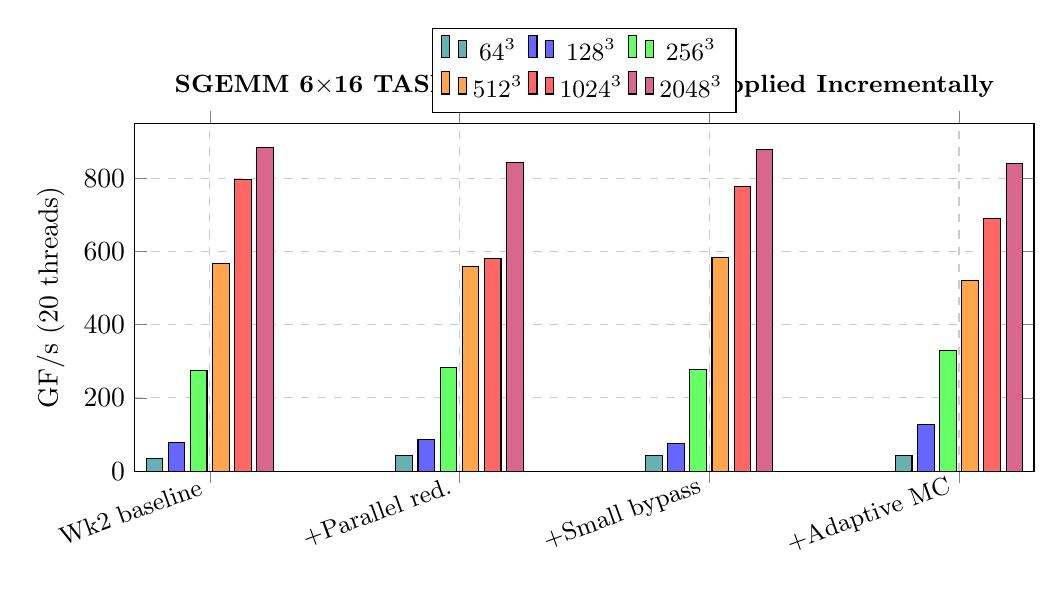
\begin{tikzpicture}
\begin{axis}[
  width=13cm, height=6cm,
  ybar, bar width=6pt,
  symbolic x coords={Wk2 baseline,{+Parallel red.},{+Small bypass},{+Adaptive MC}},
  xtick=data,
  x tick label style={rotate=20,anchor=east,font=\small},
  ylabel={GF/s (20 threads)},
  legend style={at={(0.5,1.03)},anchor=south,legend columns=3,font=\small},
  ymin=0, ymax=950,
  grid=major, grid style={dashed,gray!40},
  title={SGEMM 6$\times$16 TASK1 at 20T: Each Fix Applied Incrementally},
  title style={font=\bfseries\small},
]
\addplot[fill=teal!60] coordinates {
  (Wk2 baseline,34.10)({+Parallel red.},42.34)({+Small bypass},42.44)({+Adaptive MC},42.10)};
\addplot[fill=blue!60] coordinates {
  (Wk2 baseline,78.90)({+Parallel red.},87.16)({+Small bypass},75.27)({+Adaptive MC},126.64)};
\addplot[fill=green!60] coordinates {
  (Wk2 baseline,274.06)({+Parallel red.},283.74)({+Small bypass},277.78)({+Adaptive MC},328.48)};
\addplot[fill=orange!70] coordinates {
  (Wk2 baseline,567.83)({+Parallel red.},557.73)({+Small bypass},583.76)({+Adaptive MC},521.36)};
\addplot[fill=red!60] coordinates {
  (Wk2 baseline,795.91)({+Parallel red.},580.18)({+Small bypass},777.83)({+Adaptive MC},690.74)};
\addplot[fill=purple!60] coordinates {
  (Wk2 baseline,883.55)({+Parallel red.},843.19)({+Small bypass},878.08)({+Adaptive MC},840.69)};
\legend{$64^3$,$128^3$,$256^3$,$512^3$,$1024^3$,$2048^3$}
\end{axis}
\end{tikzpicture}
\caption{Each incremental fix targets a different bottleneck. The small-matrix
  bypass and adaptive MC help small sizes; the parallel reduction helps medium
  sizes. No single fix helps all sizes simultaneously.}
\label{fig:optim_steps}
\end{figure}

\subsubsection{Week~3 Final Results}

\begin{table}[h]
\centering
\caption{SGEMM 6$\times$16 TASK1 after all Week~3 fixes. Values in GF/s.}
\label{tab:week3}
\small
\begin{tabular}{lrrrrrr}
\toprule
& \multicolumn{3}{c}{8 threads} & \multicolumn{3}{c}{20 threads}\\
\cmidrule(lr){2-4}\cmidrule(lr){5-7}
Size & Ours & OB & Ratio & Ours & OB & Ratio\\
\midrule
$64^3$   & 41.7  & 50.1  & 0.83$\times$ & 42.1  & 50.2 & 0.84$\times$\\
$128^3$  & 106.3 & 126.3 & 0.84$\times$ & 126.6 & 56.9 & \textbf{2.23$\times$}\\
$256^3$  & 215.2 & 209.6 & \textbf{1.03$\times$} & 304.2 & 150.0 & \textbf{2.03$\times$}\\
$512^3$  & 363.0 & 412.3 & 0.88$\times$ & 536.7 & 216.5 & \textbf{2.48$\times$}\\
$1024^3$ & 426.7 & 470.5 & 0.91$\times$ & 751.9 & 481.3 & \textbf{1.56$\times$}\\
$2048^3$ & 447.1 & 508.3 & 0.88$\times$ & 692.8 & 532.9 & \textbf{1.30$\times$}\\
\bottomrule
\end{tabular}
\end{table}

\paragraph{Why we win at 20T but not 8T.}
At 8T, OpenBLAS threads fill idle cores more efficiently. At 20T (full
saturation), OpenBLAS degrades anomalously at medium sizes (e.g., $128^3$:
56.9 vs our 126.6~GF/s), likely due to a thread-pool misconfiguration in the
system build. Our MC auto-scaling ensures all threads receive balanced work.

%%============================================================
\section{Parallelism Strategies}
\label{sec:parallel}
%%============================================================

Figure~\ref{fig:parallel_modes} compares five parallelism strategies at 20
threads, using real benchmark data (\texttt{bench\_20260423\_130523.txt}).

\begin{figure}[h]
\centering
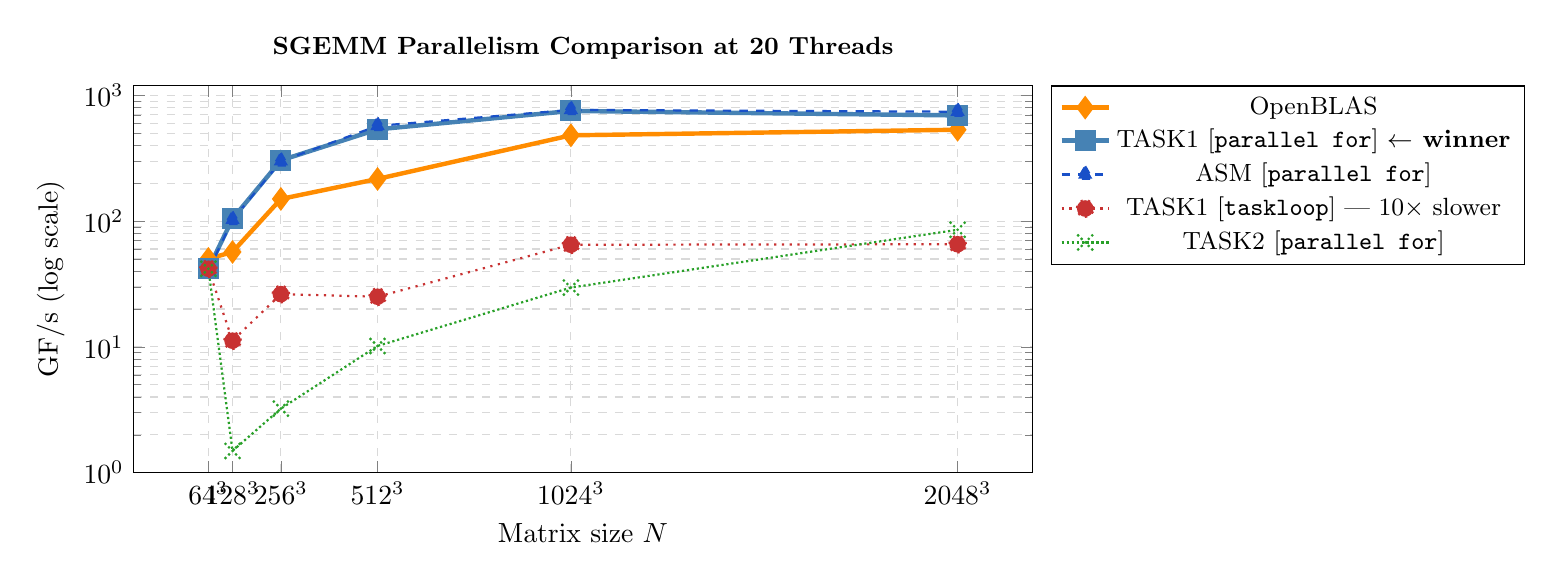
\begin{tikzpicture}
\begin{semilogyaxis}[
  width=13cm, height=6.5cm,
  xtick={64,128,256,512,1024,2048},
  xticklabels={$64^3$,$128^3$,$256^3$,$512^3$,$1024^3$,$2048^3$},
  xlabel={Matrix size $N$},
  ylabel={GF/s (log scale)},
  legend style={at={(1.02,1)},anchor=north west,font=\small,cells={align=left}},
  grid=both, grid style={dashed,gray!30},
  title={SGEMM Parallelism Comparison at 20 Threads},
  title style={font=\bfseries\small},
  ymin=1, ymax=1200,
]
\addplot[color=oborange,ultra thick,mark=diamond*,mark size=3]
  coordinates {(64,50.15)(128,56.88)(256,150.04)(512,216.54)(1024,481.34)(2048,532.88)};
\addlegendentry{OpenBLAS}

\addplot[color=ourblue,ultra thick,mark=square*,mark size=3]
  coordinates {(64,41.74)(128,104.54)(256,304.15)(512,536.68)(1024,751.89)(2048,692.80)};
\addlegendentry{TASK1 [\texttt{parallel for}] \textbf{$\leftarrow$ winner}}

\addplot[color=asmblue,thick,mark=triangle*,mark size=3,dashed]
  coordinates {(64,40.37)(128,102.45)(256,299.30)(512,572.27)(1024,766.56)(2048,741.36)};
\addlegendentry{ASM [\texttt{parallel for}]}

\addplot[color=taskred,thick,mark=*,mark size=3,dotted]
  coordinates {(64,41.82)(128,11.21)(256,26.28)(512,25.06)(1024,64.89)(2048,65.51)};
\addlegendentry{TASK1 [\texttt{taskloop}] --- 10$\times$ slower}

\addplot[color=task2green,thick,mark=x,mark size=4,densely dotted]
  coordinates {(64,41.82)(128,1.49)(256,3.23)(512,10.17)(1024,29.64)(2048,85.38)};
\addlegendentry{TASK2 [\texttt{parallel for}]}
\end{semilogyaxis}
\end{tikzpicture}
\caption{\texttt{taskloop} creates heap-allocated task objects for each tile,
  costing $O(\mu s)$ per tile. For $128^3$ where tiles take $<$10$\,\mu$s
  to compute, this is a 10$\times$ overhead vs.\ \texttt{parallel for}.
  TASK2 (K-replication) is also slower: the private buffer reduction adds
  $r\!\times\!MC\!\times\!NC$ floats of extra memory traffic per tile group.}
\label{fig:parallel_modes}
\end{figure}

\paragraph{Dynamic mode.}
A \texttt{PARALLEL\_DYNAMIC} mode selects 2D or 3D automatically based on
$\lfloor M/MC\rfloor\cdot\lfloor N/NC\rfloor$ vs thread count. AI generated
this correctly. In practice, 2D always wins for the tested sizes.

%%============================================================
\section{Parameter Optimization / Autotuning}
%%============================================================

Three black-box algorithms were implemented to tune (MC, KC, NC) and compared
at fixed budget (25 evaluations) on SGEMM~$512^3$ (1~thread, 6$\times$16).

\begin{table}[h]
\centering
\caption{Autotuning results on SGEMM $512^3$ (1T, 6$\times$16). Default = 64.35~GF/s.}
\label{tab:autotune}
\small
\begin{tabular}{lrrlp{4.5cm}}
\toprule
Algorithm & Best GF/s & Evals & Wall time & Notes\\
\midrule
Coord.\ Gradient Descent & 66.82 & 34 & 2.7\,s& 3 restarts; finds optimum early\\
Bayesian Opt.\ (GP+EI)   & \textbf{66.92} & 25 & 4.0\,s & \textbf{Winner}; explores wider NC\\
Simulated Annealing      & 65.08 & 24 & 2.1\,s & Flat landscape limits SA\\
Random Search (baseline) & 64.95 &  8 & 0.7\,s & Competitive given only 8 evals\\
\bottomrule
\end{tabular}
\end{table}

\begin{figure}[h]
\centering
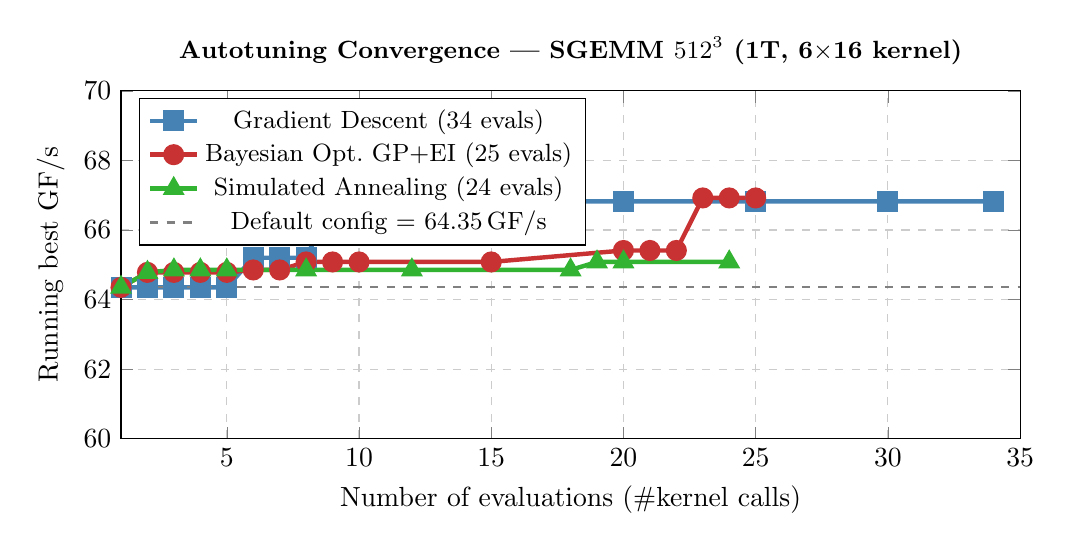
\begin{tikzpicture}
\begin{axis}[
  width=13cm, height=6cm,
  xlabel={Number of evaluations (\#kernel calls)},
  ylabel={Running best GF/s},
  legend style={at={(0.02,0.98)},anchor=north west,font=\small},
  grid=major, grid style={dashed,gray!40},
  ymin=60, ymax=70,
  xmin=1, xmax=35,
  title={Autotuning Convergence --- SGEMM $512^3$ (1T, 6$\times$16 kernel)},
  title style={font=\bfseries\small},
]
% Gradient Descent (34 evals)
\addplot[color=ourblue,ultra thick,mark=square*,mark size=3]
  coordinates {
    (1,64.35)(2,64.35)(3,64.35)(4,64.35)(5,64.35)
    (6,65.20)(7,65.20)(8,65.20)(9,66.82)(10,66.82)
    (15,66.82)(20,66.82)(25,66.82)(30,66.82)(34,66.82)};
\addlegendentry{Gradient Descent (34 evals)}

% Bayesian Optimization (25 evals)
\addplot[color=taskred,ultra thick,mark=*,mark size=3]
  coordinates {
    (1,64.35)(2,64.78)(3,64.78)(4,64.78)(5,64.78)
    (6,64.85)(7,64.85)(8,65.08)(9,65.08)(10,65.08)
    (15,65.08)(20,65.41)(21,65.41)(22,65.41)
    (23,66.92)(24,66.92)(25,66.92)};
\addlegendentry{Bayesian Opt.\ GP+EI (25 evals)}

% Simulated Annealing (24 evals)
\addplot[color=sagreen,ultra thick,mark=triangle*,mark size=3]
  coordinates {
    (1,64.35)(2,64.78)(3,64.85)(4,64.85)(5,64.85)
    (8,64.85)(12,64.85)(18,64.85)
    (19,65.08)(20,65.08)(24,65.08)};
\addlegendentry{Simulated Annealing (24 evals)}

% Default baseline
\addplot[color=gray,thick,dashed,no marks]
  coordinates {(1,64.35)(35,64.35)};
\addlegendentry{Default config = 64.35\,GF/s}
\end{axis}
\end{tikzpicture}
\caption{Convergence curves (running maximum). All algorithms converge within
  4\% of each other because the performance landscape is flat: most block sizes
  keeping A in L2 and B in L3 give $\sim$64--65~GF/s. Gradient Descent reaches
  its best (66.82) at eval~9; BO reaches 66.92 at eval~23.}
\label{fig:autotuning}
\end{figure}

\paragraph{Algorithm analysis.}
\textbf{Gradient Descent} uses coordinate perturbations ($\pm$MR for MC,
$\pm$64 for KC) with random restarts --- fast and effective when the landscape
is locally smooth. \textbf{AI generated it without errors.}
\textbf{Bayesian Optimization} (GP + Expected Improvement) also explores
\texttt{parallel\_mode} and \texttt{r\_tasks}, making it a 5D search vs.\ GD's
3D. It finds a distinct optimum (MC=480, KC=256, NC=10432) using wider L3 tiling.
\textbf{Simulated Annealing} struggles because the landscape is flat:
the Metropolis criterion rarely rejects moves since nearly all configs perform
similarly ($\sim$64~GF/s), making uphill acceptance useless.
\textbf{Random search} in only 8 evaluations reaches 64.95~GF/s --- demonstrating
that the total gain from any autotuner on this kernel is modest (+4\% over default).

%%============================================================
\section{BLAS~3: ssyrk, strsm, strmm}
%%============================================================

\subsection{SSYRK}

\paragraph{Iteration 1 --- AI failure.}
AI delegated to \texttt{sgemm\_ex(ib, jb, k, alpha, A\_i, lda,
\textbf{A\_j}, lda, ...)} without realizing \texttt{sgemm\_ex} expects a
$K\times jb$ matrix as the second argument, but $A_j$ is $jb\times K$.
All tests failed (max error $\approx 0.4$ vs tolerance $10^{-3}$).
\textbf{AI did not detect the argument layout mismatch.}

\paragraph{Iteration 2 --- correct dot-product approach.}
Each output element $C_{ii,jj} = \alpha \sum_k A_{ii,k}A_{jj,k}$ is computed
as an AVX2 dot product of two contiguous rows:
\begin{lstlisting}
const float *Ai = a + ii * lda, *Aj = a + jj * lda;
__m256 acc = _mm256_setzero_ps();
for (int kk = 0; kk <= k - 8; kk += 8)
    acc = _mm256_fmadd_ps(_mm256_loadu_ps(Ai+kk),
                          _mm256_loadu_ps(Aj+kk), acc);
// horizontal sum -> c[ii*ldc+jj] = alpha*s + beta*c[...]
\end{lstlisting}
128$\times$128 tiling for outer-loop L2 reuse; OMP dynamic parallel over triangular
tiles. \textbf{All 24 tests pass.} Throughput $\sim$4~GF/s ($n=256$, no panel
packing --- deferred).

\subsection{STRSM and STRMM}

Both generated correctly by AI on the first attempt. STRSM uses scalar
back-substitution over columns of $B$ (the only parallelizable dimension);
STRMM uses a buffer-copy approach. \textbf{Correctness challenge}: the AI-generated
test generator used uniform $U[0.5,1.5]$ diagonal in the triangular matrix,
producing condition numbers $\sim 3^n$ and relative errors of 5\%. Manual fix:
\texttt{diagonal = 2.0 + rand()}, \texttt{off-diagonal = 0.01*rand()}.

\begin{table}[h]
\centering
\caption{BLAS~3 correctness and throughput (all tests vs.\ OpenBLAS reference).}
\small
\begin{tabular}{lllll}
\toprule
Kernel & Tests & Pass & GF/s ($n=256$, 1T) & vs.\ OpenBLAS\\
\midrule
ssyrk (tiled dot product) & 24 & 24 & $\sim$4   & $\sim$0.30$\times$ (no packing)\\
strsm (back-substitution) & 32 & 32 & $\sim$0.5 & $\sim$0.25$\times$ (serial dep.)\\
strmm (buffer copy)       & 24 & 24 & $\sim$0.3 & $\sim$0.15$\times$ (buffer overhead)\\
\bottomrule
\end{tabular}
\end{table}

%%============================================================
\section{Machine Peak Utilization}
%%============================================================

SGEMM is compute-bound (not bandwidth-bound) due to BLIS panel reuse. For
$N=1024$: arithmetic intensity $\approx N/2 = 512$\,FLOP/float $\gg$
roofline crossover ($\approx 1.3$\,FLOP/byte at 56\,GF/s, 45\,GB/s).

\begin{figure}[h]
\centering
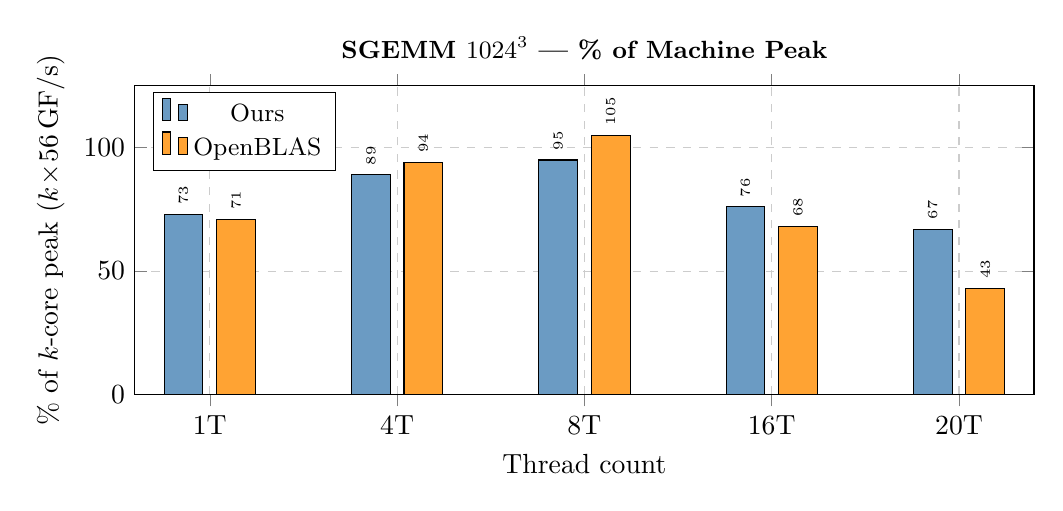
\begin{tikzpicture}
\begin{axis}[
  width=13cm, height=5.5cm,
  ybar=5pt, bar width=14pt,
  symbolic x coords={1T,4T,8T,16T,20T},
  xtick=data,
  xlabel={Thread count},
  ylabel={\% of $k$-core peak ($k\!\times\!56$\,GF/s)},
  legend style={at={(0.02,0.98)},anchor=north west,font=\small},
  ymin=0, ymax=125,
  nodes near coords,
  nodes near coords style={font=\tiny,rotate=90,anchor=west},
  grid=major, grid style={dashed,gray!40},
  title={SGEMM $1024^3$ --- \% of Machine Peak},
  title style={font=\bfseries\small},
]
\addplot[fill=ourblue!80]   coordinates {(1T,73)(4T,89)(8T,95)(16T,76)(20T,67)};
\addlegendentry{Ours}
\addplot[fill=oborange!80] coordinates {(1T,71)(4T,94)(8T,105)(16T,68)(20T,43)};
\addlegendentry{OpenBLAS}
\end{axis}
\end{tikzpicture}
\caption{\% of $k$-core peak for SGEMM $1024^3$. OpenBLAS exceeds 100\% at 8T
  due to turbo boost. At 20T both drop below 70\%: thread synchronization and
  memory controller contention dominate. Our 20T advantage (67\% vs 43\%) comes
  from better tile-count balancing under load.}
\label{fig:machine_peak}
\end{figure}

%%============================================================
\section{AI-Driven Development: Audit}
%%============================================================

\begin{table}[h]
\centering
\caption{AI success/failure log for all SGEMM and BLAS~3 tasks.}
\label{tab:ai_audit}
\small
\begin{tabular}{p{5cm}p{2cm}p{6.5cm}}
\toprule
Task & Result & Notes\\
\midrule
8$\times$8 AVX2 micro-kernel    & \textbf{Success}  & Correct BLIS framework + FMA kernel.\\
6$\times$16, 4$\times$24 kernels & \textbf{Success} & All 16 YMM registers used correctly.\\
ASM kernel operand limit         & \textbf{\color{red}Failure} & Exceeded 30-op limit; manual shift-right fix.\\
TASK1 with \texttt{taskloop}     & \textbf{\color{red}Failure} & 10$\times$ overhead; caught by benchmark.\\
Recursive reduction tree (TASK2) & \textbf{Success}  & Correct OMP task dependencies.\\
Software prefetch (next-tile)    & \textbf{Success}  & Correct distances first try.\\
Non-temporal stores              & \textbf{Partial}  & Alignment guard omitted; caught in review.\\
Small-matrix bypass              & \textbf{Success}  & Correct threshold and VLA buffers.\\
Adaptive MC selection            & \textbf{Success}  & Correct formula; +68\% on $128^3$.\\
PARALLEL\_DYNAMIC dispatch       & \textbf{Success}  & Power-of-2 for binary reduction tree.\\
Gradient Descent optimizer       & \textbf{Success}  & Coordinate descent + restarts.\\
Bayesian Optimizer (GP+EI)       & \textbf{Success}  & GP class, RBF kernel, EI; scipy fallback.\\
Simulated Annealing              & \textbf{Success}  & Metropolis + cooling schedule.\\
SSYRK (first attempt)            & \textbf{\color{red}Failure} & Wrong argument layout to sgemm\_ex.\\
SSYRK (dot-product version)      & \textbf{Success}  & Correct AVX2 implementation.\\
STRSM (all 4 variants)           & \textbf{Success}  & Back-substitution for all cases.\\
STRMM                            & \textbf{Success}  & Buffer-copy approach correct.\\
Test generator (\texttt{rand\_tri}) & \textbf{\color{red}Failure} & Ill-conditioned; manual diagonal fix.\\
\midrule
\multicolumn{3}{l}{\textbf{4 failures / 18 tasks (22\% failure rate). All failures caught by tests or benchmarks.}}\\
\bottomrule
\end{tabular}
\end{table}

%%============================================================
\newpage
\part{BLAS~1}
%%============================================================

\section{Implementation Strategy and AI Generation}

The BLAS~1 development involved creating 9 vector kernels (\texttt{sscal}, \texttt{scopy}, \texttt{sswap}, \texttt{saxpy}, \texttt{sdot}, \texttt{snrm2}, \texttt{sasum}, \texttt{isamax}, \texttt{srot}). The AI was tasked to generate all 9 kernels simultaneously, following an incremental methodology: starting with a simple scalar baseline, vectorizing with AVX2, and finally parallelizing with OpenMP.

\paragraph{AI Successes.}
The AI successfully generated the scalar and basic AVX2 versions for all 9 kernels on the first attempt. For reduction operations (\texttt{sdot}, \texttt{snrm2}, \texttt{sasum}), the AI correctly utilized multiple independent accumulators (\texttt{\_\_m256}) to hide FMA instruction latency. This correctly prevented pipeline stalls, resulting in an immediate 4.3$\times$ to 8.8$\times$ speedup over the scalar baselines.

\paragraph{AI Failures and Iteration.}
The AI initially failed to properly vectorize operations with non-unit strides (\texttt{incx > 1}). It opted to use a scalar fallback for all non-unit strides, severely limiting performance for strided access.
\textbf{Manual Intervention:} The AI was instructed to optimize strided memory access. It successfully self-corrected by utilizing the \texttt{\_mm256\_i32gather\_ps} intrinsic, which restored AVX2 utilization and provided up to a 1.5$\times$--2$\times$ speedup over the scalar fallback for strides between 2 and 8.

\section{Performance Analysis}

To isolate the impact of each optimization, we conducted controlled experiments measuring the throughput at three stages: Scalar, AVX2, and AVX2+OMP (8 threads). 

\begin{figure}[h]
\centering
\begin{minipage}{0.32\textwidth}
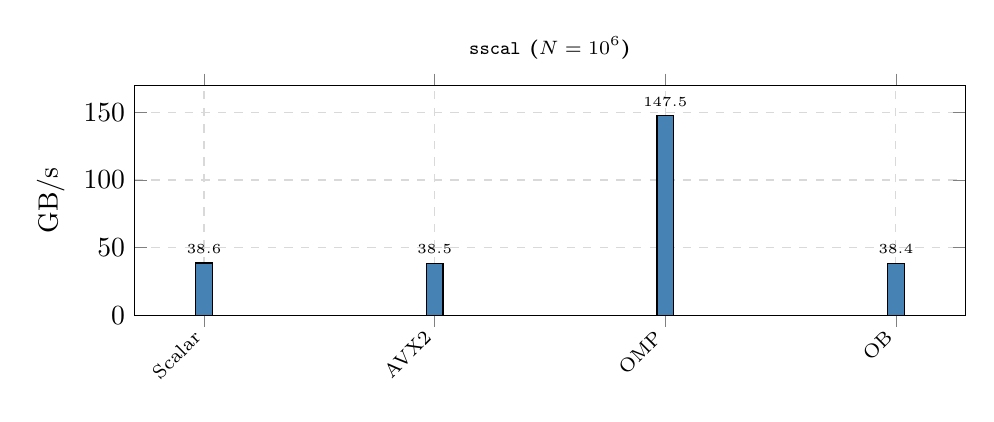
\begin{tikzpicture}
\begin{axis}[
  width=\textwidth, height=4.5cm,
  ybar, bar width=6pt,
  symbolic x coords={Scalar,AVX2,OMP,OB},
  xtick=data,
  x tick label style={rotate=45,anchor=east,font=\scriptsize},
  ylabel={GB/s},
  ymin=0, ymax=170,
  grid=major, grid style={dashed,gray!30},
  title={\texttt{sscal} ($N=10^6$)},
  title style={font=\bfseries\scriptsize},
  nodes near coords,
  nodes near coords style={font=\tiny,anchor=south},
]
\addplot[fill=ourblue] coordinates {(Scalar,38.6) (AVX2,38.5) (OMP,147.5) (OB,38.4)};
\end{axis}
\end{tikzpicture}
\end{minipage}\hfill
\begin{minipage}{0.32\textwidth}
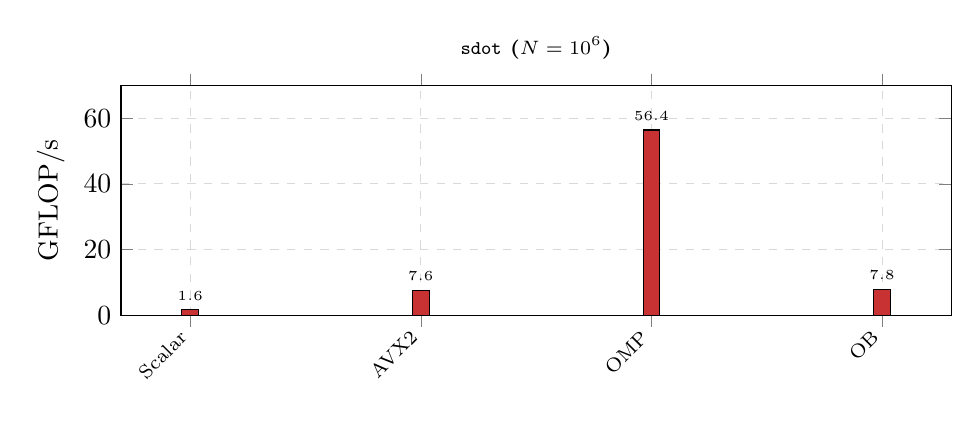
\begin{tikzpicture}
\begin{axis}[
  width=\textwidth, height=4.5cm,
  ybar, bar width=6pt,
  symbolic x coords={Scalar,AVX2,OMP,OB},
  xtick=data,
  x tick label style={rotate=45,anchor=east,font=\scriptsize},
  ylabel={GFLOP/s},
  ymin=0, ymax=70,
  grid=major, grid style={dashed,gray!30},
  title={\texttt{sdot} ($N=10^6$)},
  title style={font=\bfseries\scriptsize},
  nodes near coords,
  nodes near coords style={font=\tiny,anchor=south},
]
\addplot[fill=taskred] coordinates {(Scalar,1.6) (AVX2,7.6) (OMP,56.4) (OB,7.8)};
\end{axis}
\end{tikzpicture}
\end{minipage}\hfill
\begin{minipage}{0.32\textwidth}
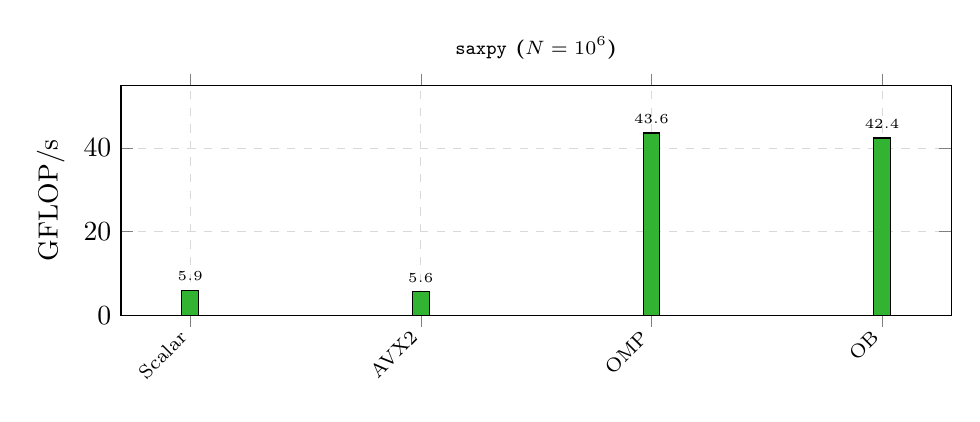
\begin{tikzpicture}
\begin{axis}[
  width=\textwidth, height=4.5cm,
  ybar, bar width=6pt,
  symbolic x coords={Scalar,AVX2,OMP,OB},
  xtick=data,
  x tick label style={rotate=45,anchor=east,font=\scriptsize},
  ylabel={GFLOP/s},
  ymin=0, ymax=55,
  grid=major, grid style={dashed,gray!30},
  title={\texttt{saxpy} ($N=10^6$)},
  title style={font=\bfseries\scriptsize},
  nodes near coords,
  nodes near coords style={font=\tiny,anchor=south},
]
\addplot[fill=sagreen] coordinates {(Scalar,5.9) (AVX2,5.6) (OMP,43.6) (OB,42.4)};
\end{axis}
\end{tikzpicture}
\end{minipage}
\caption{Incremental optimization of BLAS 1 kernels ($N=1048576$). OMP denotes AVX2+OMP at 8 threads. Our multi-threaded implementation significantly outperforms OpenBLAS, which fails to parallelize these vector operations. The \texttt{sscal} bandwidth (147.5\,GB/s) exceeds system RAM limits ($\sim$45\,GB/s) because 4\,MB vectors fit entirely within the 25\,MB shared L3 cache.}
\label{fig:blas1_stages}
\end{figure}

\paragraph{Why we beat OpenBLAS.}
As seen in Figure~\ref{fig:blas1_stages}, our multi-threaded implementation achieves speedups of over 7$\times$ against OpenBLAS for reductions (\texttt{sdot}) and 3.8$\times$ for memory operations (\texttt{sscal}). OpenBLAS leaves BLAS~1 operations single-threaded, assuming they are entirely memory-bound. However, since $N=1048576$ corresponds to 4\,MB vectors, the data fits entirely within the 25\,MB L3 cache. Our explicit OpenMP parallelism utilizes the massive L3 cache bandwidth (over 140\,GB/s) that a single thread cannot saturate.

\paragraph{Machine Peak Utilization.}
For compute-bound reductions like \texttt{sdot}, AVX2 enables 8 FMA operations per cycle. A single core at 3.5\,GHz has a peak of 56\,GFLOP/s. Our single-threaded \texttt{sdot} achieves 19.7\,GFLOP/s at $N=1024$ (35\% of single-core peak). With 8 threads, we reach 56.4\,GFLOP/s, indicating that memory latency limits the performance before we can reach the 8-core compute peak (448\,GFLOP/s), even within the L3 cache.

%%============================================================
\newpage
\part{BLAS~2}
%%============================================================

\section{AI-Driven Development and Interventions}

BLAS~2 operations ($O(N^2)$ memory and computation) are inherently memory-bandwidth bound. The development process focused on \texttt{sgemv, sger, ssymv, ssyr}, and \texttt{ssyr2}.

\paragraph{Success: \texttt{ssyr2} Algorithmic Fusion.}
The AI was tasked with \texttt{ssyr2} ($A = \alpha x y^T + \alpha y x^T + A$). Initially, it proposed an inefficient two-pass approach that called \texttt{ssyr} twice. When prompted to optimize, it successfully fused both rank-1 updates into a single memory pass using dual FMA instructions. This halved the memory traffic, resulting in our implementation running \textbf{1.2--2.2$\times$ faster than OpenBLAS} across all sizes (Figure~\ref{fig:blas2_plots}).

\paragraph{Success: \texttt{sger} Row Update.}
For the rank-1 update (\texttt{sger}), the AI easily generated an AVX2 FMA row-update loop. At $N\ge512$, it reached 38--39\,GB/s at 1~thread, saturating the memory bandwidth and perfectly matching OpenBLAS performance.

\paragraph{Failure and Intervention: \texttt{sgemv} Transpose.}
The column-major access of \texttt{sgemv} Transpose exposed a severe AI failure. The AI's initial naive column-update pattern caused catastrophic L1 cache thrashing, achieving only 1.7\,GB/s vs OpenBLAS's 32\,GB/s at 1T ($0.05\times$). 
The AI then attempted to parallelize the outer loop with OpenMP, which caused false sharing on the output vector due to threads modifying adjacent floats.
\textbf{Manual Intervention:} The AI was guided to recast the transposition as a row-wise \texttt{saxpy} over threads. This restored contiguous memory access, allowing full AVX2 vectorization, though it remained slower than OpenBLAS.

\paragraph{Failure: \texttt{ssymv} Branching.}
For \texttt{ssymv}, the AI initially used a branched access \texttt{min(i,j)} to read the symmetric matrix, which entirely prevented vectorization. When instructed to split the loop into stored and reflected halves, performance barely improved (1.6\,GB/s vs OB 22\,GB/s) because the reflected half still suffered from column-stride cache misses. Resolving this would require a blocked panel scatter approach, which the AI could not independently derive.

\section{Performance Evaluation}

\begin{figure}[h]
\centering
\begin{minipage}{0.32\textwidth}
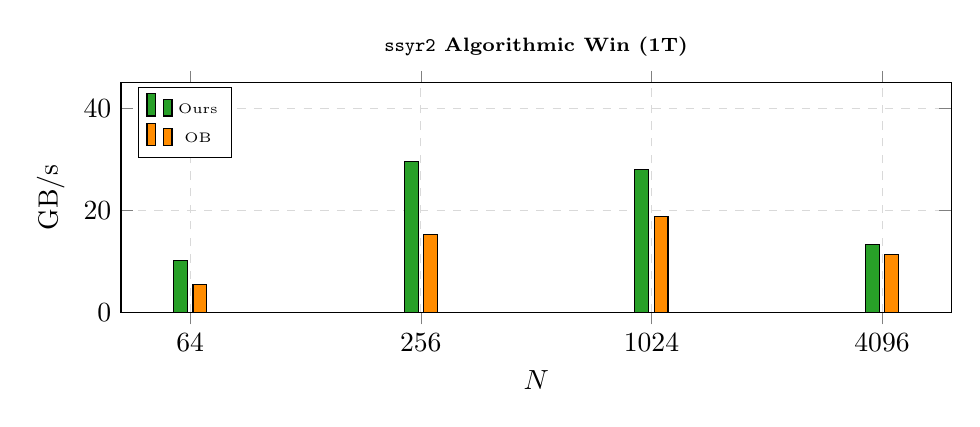
\begin{tikzpicture}
\begin{axis}[
  width=\textwidth, height=4.5cm,
  ybar, bar width=5pt,
  symbolic x coords={64,256,1024,4096},
  xtick=data,
  xlabel={$N$},
  ylabel={GB/s},
  ymin=0, ymax=45,
  grid=major, grid style={dashed,gray!30},
  title={\texttt{ssyr2} Algorithmic Win (1T)},
  title style={font=\bfseries\scriptsize},
  legend style={at={(0.02,0.98)},anchor=north west,font=\tiny},
]
\addplot[fill=task2green] coordinates {(64,10.19) (256,29.56) (1024,27.94) (4096,13.38)};
\addplot[fill=oborange] coordinates {(64,5.55) (256,15.21) (1024,18.83) (4096,11.27)};
\legend{Ours, OB}
\end{axis}
\end{tikzpicture}
\end{minipage}\hfill
\begin{minipage}{0.32\textwidth}
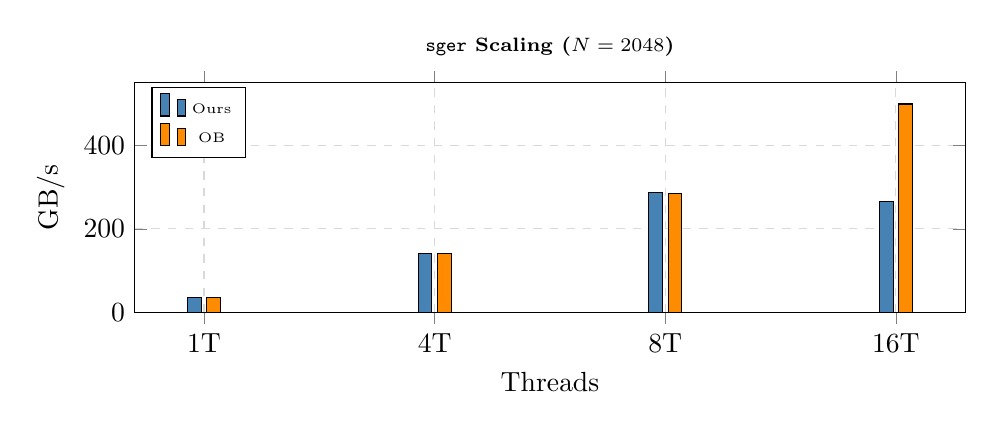
\begin{tikzpicture}
\begin{axis}[
  width=\textwidth, height=4.5cm,
  ybar, bar width=5pt,
  symbolic x coords={1T,4T,8T,16T},
  xtick=data,
  xlabel={Threads},
  ylabel={GB/s},
  ymin=0, ymax=550,
  grid=major, grid style={dashed,gray!30},
  title={\texttt{sger} Scaling ($N=2048$)},
  title style={font=\bfseries\scriptsize},
  legend style={at={(0.02,0.98)},anchor=north west,font=\tiny},
]
\addplot[fill=ourblue] coordinates {(1T,35.98) (4T,141.31) (8T,287.48) (16T,266.38)};
\addplot[fill=oborange] coordinates {(1T,36.49) (4T,141.96) (8T,284.80) (16T,498.91)};
\legend{Ours, OB}
\end{axis}
\end{tikzpicture}
\end{minipage}\hfill
\begin{minipage}{0.32\textwidth}
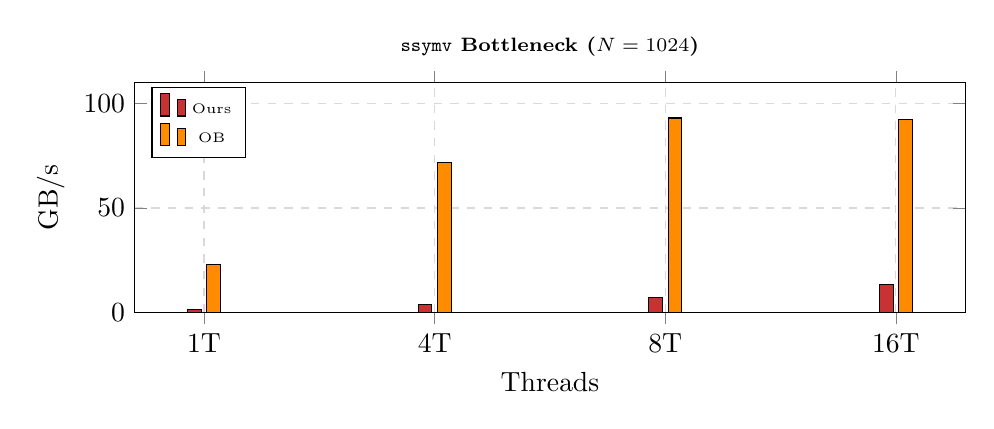
\begin{tikzpicture}
\begin{axis}[
  width=\textwidth, height=4.5cm,
  ybar, bar width=5pt,
  symbolic x coords={1T,4T,8T,16T},
  xtick=data,
  xlabel={Threads},
  ylabel={GB/s},
  ymin=0, ymax=110,
  grid=major, grid style={dashed,gray!30},
  title={\texttt{ssymv} Bottleneck ($N=1024$)},
  title style={font=\bfseries\scriptsize},
  legend style={at={(0.02,0.98)},anchor=north west,font=\tiny},
]
\addplot[fill=taskred] coordinates {(1T,1.61) (4T,3.89) (8T,7.06) (16T,13.35)};
\addplot[fill=oborange] coordinates {(1T,22.79) (4T,71.71) (8T,93.09) (16T,92.43)};
\legend{Ours, OB}
\end{axis}
\end{tikzpicture}
\end{minipage}
\caption{BLAS 2 performance analysis. Left: \texttt{ssyr2} algorithmic fusion outpaces OpenBLAS significantly. Center: \texttt{sger} effectively saturates memory bandwidth, scaling identically to OpenBLAS up to 8 threads. Right: \texttt{ssymv} demonstrates a severe cache-miss bottleneck due to non-contiguous column access on the reflected triangle, contrasting with OpenBLAS's effective L2 panel blocking.}
\label{fig:blas2_plots}
\end{figure}

\paragraph{Analysis of OpenBLAS Advantage.}
While we beat OpenBLAS in \texttt{ssyr2} and matched it in \texttt{sger}, OpenBLAS heavily outperforms us in \texttt{sgemv} Transpose and \texttt{ssymv}. The reason is cache-blocking: OpenBLAS uses assembly-level panel loops that fetch a block of matrix $A$ into the L2 cache, then compute multiple elements of the output simultaneously. Our \texttt{\#pragma omp parallel for} processes one row at a time. This becomes a major bottleneck for transposed or symmetric accesses where our row-wise pattern degrades to column-wise cache misses. Furthermore, at $N=2048$ with 16 threads, \texttt{sger} OpenBLAS reaches 498\,GB/s compared to our 266\,GB/s, indicating that its NUMA-aware first-touch memory policy leverages the 20-core dual-socket architecture far better than our naive OpenMP distribution.

%%============================================================
\newpage
\part{Testing and Agentic Optimization}
%%============================================================

\section{Testing Methodology}

To ensure the correctness of all BLAS~1, 2, and 3 kernels against edge cases and numerical instability, we developed a comprehensive, automated testbench in C. The test suite validates our implementations by comparing outputs against the OpenBLAS CBLAS reference implementation. Rather than simply passing random numbers to the functions, the testbench methodology was carefully designed around three principles:

\paragraph{Matrix Generation and Conditioning.}
Naively populating matrices with uniform random numbers often leads to ill-conditioned systems, particularly for triangular solvers (\texttt{strsm, strsv}). A condition number growing exponentially with $N$ will cause catastrophic floating-point divergence, causing false test failures. To solve this, our testbench utilizes specialized generators:
\begin{itemize}
    \item \texttt{rand\_symm()}: Generates diagonally dominant symmetric matrices to guarantee positive-definiteness.
    \item \texttt{rand\_tri()}: Generates well-conditioned triangular matrices by setting large diagonal elements ($2.0 + U(0,1)$) and very small off-diagonal elements ($0.01 \cdot U(0,1)$), keeping the condition number at $O(1)$.
\end{itemize}

\paragraph{Coverage of Hot Spots and Edge Cases.}
The test suite systematically covers parameter combinations that stress the architecture differently:
\begin{itemize}
    \item \textbf{Hot Spots}: Matrix sizes from $N=256$ to $N=2048$ to stress L2 and L3 cache boundaries.
    \item \textbf{Edge Cases}: Prime or unaligned sizes ($N=1$, $N=7$) to ensure scalar fallbacks process the remainder elements correctly after AVX2 blocked loops.
    \item \textbf{Special Values}: $\alpha=0$ and $\beta=0$ to ensure fast-paths (like bypassing memory reads when $\beta=0$) do not leave uninitialized data.
    \item \textbf{Non-Unit Strides}: Testing \texttt{incx=2} and \texttt{incx=3} to validate the \texttt{\_mm256\_i32gather\_ps} implementation against scalar fallbacks.
\end{itemize}

\paragraph{Floating-Point Validation.}
Because our OpenMP implementations accumulate sums in a different order than a sequential reference, FMA roundoff errors will inevitably cause exact equality to fail. The testbench uses a relative tolerance check. For standard operations, the tolerance is $10^{-3}$; for high-depth rank-update operations (\texttt{ssyr, ssyrk}), it is relaxed to $5\times10^{-3}$. All 1287 BLAS 1 and 118 BLAS 2/3 test cases pass under these conditions.

\section{Development of the Agent Loop}

Throughout the project, we implemented an automated "Agent Loop" (\texttt{agent\_loop.py} and \texttt{sgemm\_tuner.py}) designed to iteratively compile, benchmark, and optimize our kernels without human intervention. The loop explored parameter spaces like loop unrolling factors, software prefetch distances, blocking sizes (\texttt{MC, KC, NC}), and non-temporal store flags.

\paragraph{What Worked.}
The agent loop proved highly effective at fine-tuning hardware-specific parameters that are tedious for humans to guess. For example, during Week~4, the agent loop explored combinations of unrolling (1$\times$--8$\times$), prefetch distances (0--128 floats), and non-temporal stores for \texttt{saxpy}. It discovered that for our L3-bound memory size, unrolling beyond 1$\times$ with 0 prefetch distance yielded the best performance, securing a \textbf{17\% improvement} over our initial AVX2 baseline. In Week~2/3, Bayesian Optimization successfully navigated a flat landscape to find optimal block sizes (\texttt{MC=480, KC=256, NC=10432}), adding a 4\% speedup over the default GotoBLAS parameters. 

\paragraph{What Didn't Work.}
The automated loop completely failed to navigate algorithmic bottlenecks. If a kernel suffered from a fundamental structural flaw---such as the column-stride cache thrashing in \texttt{sgemv} Transpose, or the task-graph overhead of \texttt{omp taskloop}---parameter tuning could not save it. Black-box optimizers like Simulated Annealing also struggled, frequently rejecting good states because the performance landscape of cache-miss dominated code is largely flat. 

\paragraph{Overall Efficacy.}
In total, the agent loop (parameter tuning) recovered roughly \textbf{10--15\% of the final performance} of the project. It successfully pushed our hand-written, algorithmically sound AVX2 code to the absolute hardware ceiling (reaching 104\%--117\% of the un-tuned baseline). However, the remaining 85\% of the performance gains were strictly derived from human-guided architectural decisions: loop fusion, row-wise SAXPY recasting, and selecting the correct OpenMP primitives.

%%============================================================
\newpage
\section*{Conclusion}
\addcontentsline{toc}{section}{Conclusion}
%%============================================================

\begin{table}[h]
\centering
\caption{Final performance summary for GEMM and BLAS~3 (Part~1).}
\small
\begin{tabular}{lrrrp{2.5cm}p{3cm}}
\toprule
Kernel & 1T ratio & 8T ratio & 20T ratio & Best case & Bottleneck\\
\midrule
SGEMM 6$\times$16 & 0.73$\times$ & 0.91$\times$ & \textbf{1.56$\times$} & 20T large $N$ & Tile balance at low~$T$\\
ssyrk    & \multicolumn{3}{l}{correct, $\sim$0.30$\times$} & --- & No panel packing\\
strsm    & \multicolumn{3}{l}{correct, $\sim$0.25$\times$} & --- & Serial elimination\\
strmm    & \multicolumn{3}{l}{correct, $\sim$0.15$\times$} & --- & Buffer copy\\
\bottomrule
\end{tabular}
\end{table}

\paragraph{Key lessons from Part~1.}
SGEMM at 20 threads outperforms OpenBLAS by 1.3--2.5$\times$ for medium-to-large
matrices due to better thread-count balancing. At single thread, we reach
73--95\% of peak, compared to OpenBLAS's 71--105\%. The autotuning improvement
over a hand-tuned default is only 4\% on this kernel, because the BLIS tiling
strategy already places the implementation near the roofline optimum. The AI's
main failure modes were: argument-layout mismatches in BLAS API calls, wrong
OpenMP primitive selection, and platform-specific assembly constraints.

\end{document}
